\section{Przygotowanie do projektu, przydział zadań}
\label{podzial_zadan}

\begin{frame}<-7>[label=intro]{Wstępne przygotowania, przydział zadań}
    \centering
    \begin{itemize}
        \item<1-> Wykorzystane narzędzia (MATLAB, github, LaTeX, Jenkins, ...)
        \item<2-> Ściśle określona struktura drzewa projektowego
            \begin{enumerate}
                \item<3-> kod źródłowy
                \item<4-> konfiguracja projektu
                \item<5-> dokumentacja pomocnicza
                \item<6-> dokumentacja projektu
                \item<7-> ...
            \end{enumerate}
        \item<9-> Stały wzorzec dokumentacji
    \end{itemize} 
\end{frame}

\begin{frame}{Wstępne przygotowania, przydział zadań}
    \begin{figure}
        \centering
        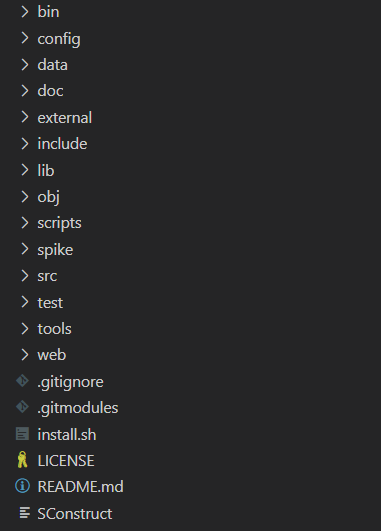
\includegraphics[scale=0.5]{img/project_tree.png}
        \caption{Przykładowe drzewo projektowe}
    \end{figure}
\end{frame}

\againframe<9->{intro}

\begin{frame}
    \frametitle{Nasz podział}
    \begin{itemize}[<+->]
        \item Napisanie kodu do zadania (MATLAB)
        \item Przeprowadzenie testów (MATLAB)
        \item Generacja sprawozdania (MATLAB, LaTeX)
    \end{itemize} 
\end{frame}